\definecolor{turkis}{RGB}{100, 253, 205}

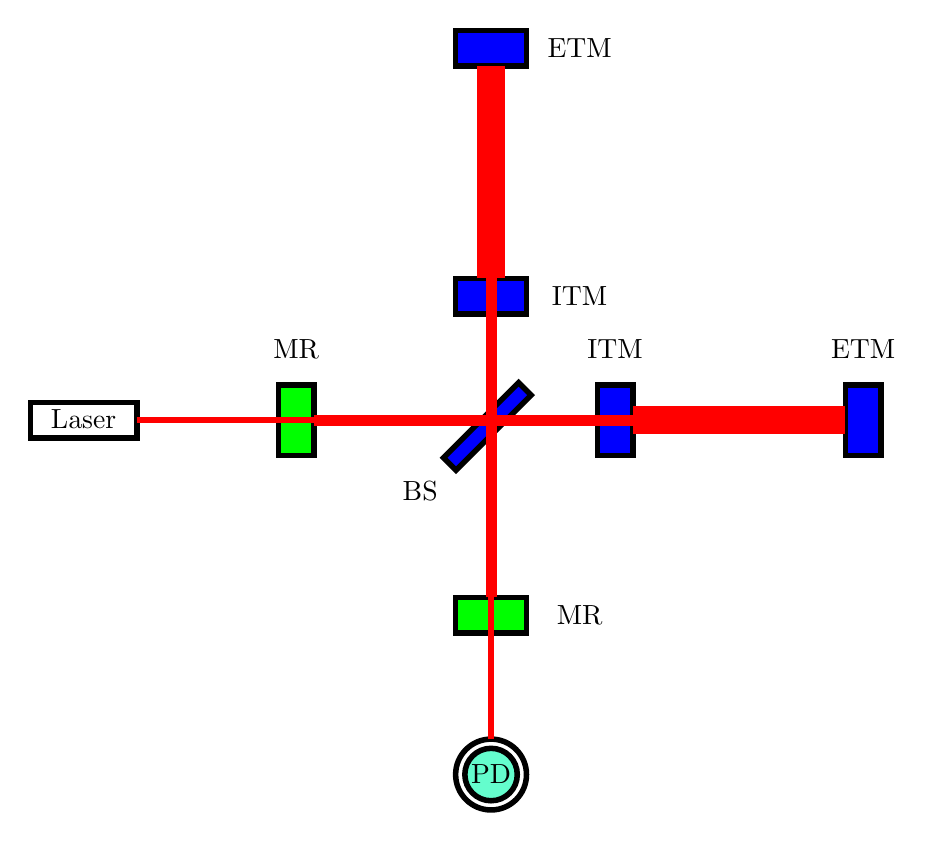
\begin{tikzpicture}[scale=0.9]

% Laser
\draw[line width=2pt] (-6.5,-0.25) rectangle ++(1.5,0.5);
\node[align=center] at (-5.75,0.02) {Laser};

% Beam splitter
\draw[line width=2pt, fill=blue, rotate=-45] (-0.1,-0.85) rectangle ++(0.25,1.5);
\node[align=center] at (-1,-1) {BS};

% ETM
\draw[line width=2pt, fill=blue] (-0.5,5) rectangle ++(1,0.5);
\draw[line width=2pt, fill=blue] (5,-0.5) rectangle ++(0.5,1);
\node[align=center] at (1.25,5.25) {ETM};
\node[align=center] at (5.25,1) {ETM};

%ITM
\draw[line width=2pt, fill=blue] (-0.5,1.5) rectangle ++(1,0.5);
\draw[line width=2pt, fill=blue] (1.5,-0.5) rectangle ++(0.5,1);
\node[align=center] at (1.25,1.75) {ITM};
\node[align=center] at (1.75,1) {ITM};

%Modulation & Recycling
\draw[line width=2pt, fill=green] (-0.5,-3) rectangle ++(1,0.5);
\draw[line width=2pt, fill=green] (-3,-0.5) rectangle ++(0.5,1);
\node[align=center] at (1.25,-2.75) {MR};
\node[align=center] at (-2.75,1) {MR};

% Detector
\fill[color=turkis] (0, -5) circle (0.4);
\draw[line width=2pt] (0, -5) circle(0.37);
\draw[line width=2pt] (0, -5) circle(0.5);
\node[align=center] at (0,-5) {PD};

% Beam paths
\draw[line width=2pt, color=red] (0,-4.5) -- (0,5);
\draw[line width=2pt, color=red] (-5,0) -- (5,0);
\draw[line width=4pt, color=red] (0,-2.5) -- (0,2);
\draw[line width=4pt, color=red] (-2.5,0) -- (2,0);
\draw[line width=10pt, color=red] (0,2) -- (0,5);
\draw[line width=10pt, color=red] (2,0) -- (5,0);

\end{tikzpicture}